\chapter{Cylindrical Simulations to Study the Effect of Beam Radius in Direct-Drive}

This chapter describes a cylindrical, direct-drive implosion simulation platform and corresponding ensemble of simulations that was developed to study the effect of the beam radius initial condition on \textsc{Omega} laser facility experiments.
Although results from the cylindrical simulations do not have the same convergence properties of spherical implosions, much of the essential physics which is important to studying the effect of beam radius is preserved.
The main benefit of the geometry is that a 2-D ray-trace can be used to model the lasers which yields several orders of magnitude speed up, compared to spherical 3-D implosions.
The reduction in computational expense allows ensembles of \ac{CBET} simulations to be performed, which would be exceedingly expensive for 3-D spherical calculations.
Beam radius strongly effects \ac{CBET} and therefore including a model for the interaction in computational studies is crucial.

The chapter begins with a review of the work which has been done to study the beam radius initial condition for direct-drive implosions, with an emphasis on the use of this parameter in statistical modelling of \textsc{Omega} campaigns.
A description of the cylindrical platform is then provided, which includes a discussion of its advantages, weaknesses and applicability to current \textsc{Omega} experiments.
The tuning procedure which was followed to obtain hydrodynamically similar implosions at different beam radii is then described.
The main results of the chapter are then presented, which include calculations of the power deposition asymmetry both with and without \ac{CBET} and an explanation of why \ac{CBET} typically amplifies the asymmetry.
\ac{CBET} is also shown to introduce \textit{modal flips} of the deposition in time.
Stagnation state asymmetries of the hydrodynamic profiles are then studied for all implosions and these demonstrate that while increasing beam radius in the absence of \ac{CBET} reduces beam-mode asymmetries, the opposite behaviour is observed in the presence of \ac{CBET}, although the exact relationship proves is complex.
The chapter concludes with a summary of the work and suggestions of further work that could be undertaken using the same cylindrical platform.

\newpage

%###############################################################################################################################
%###############################################################################################################################
%###############################################################################################################################
\section{Introduction to Beam Radius in Direct-Drive Inertial Confinement Fusion}%
\label{sec:Res1_Beamrad_intro}

\begin{figure}[t!]
    \includegraphics[width=\linewidth]{Results1/Images/RbRt_beam_overlap_alt.png}
    \centering
    \caption{The trajectory of rays from two beams with Beam radii.
    The density profile for both simulations is $n_e=n_{\text{cr}}\exp{[ -(r_{\mu\text{m}}-20)/100 ]}$.
    Panels a) and b) plot rays from beams with widths $\sigma=10$ and $18\ \mu\text{m}$ respectively.
    Ray trajectories are separated for each beam by colour depending on their sheet.
    Red and dark blue rays are from the incident sheet (before the ray caustic) and magenta and light blue rays are from the reflected sheet (after the ray caustic).}%
    \label{fig:Res1_RbRt_beam_overlap}
\end{figure}

An idealised direct drive implosion, (neglecting the effect of random or otherwise, shot-to-shot variations) has a limited number of initial conditions which define the implosion.
The target can be described by a set of materials and their thicknesses.
Initial target parameters are intimately coupled to the physics of the implosion and, in part, dictate the propagation time of shocks through the target, hydrodynamic stability and absorption of the laser energy.
The pulse shape describes the laser power which is incident of the target as a function of time.
This can be designed to, for example, drive shocks by introducing sharp rises in the incident power with time, which leads to sharp gradients in ablation pressure~\cite{scott_shock-augmented_2022}.
A given facility also has a number of beam ports each of which has a specific origin and pointing location, which influence the magnitude of the \textit{beam-mode} asymmetry, which arises from the uniformity of laser absorption.
The intensity profile of each laser and specifically the beam radius is an additional parameter which can be varied and plays an important role in defining both the power which can be coupled to the target and the magnitude of beam-mode asymmetry.

As shall be explored in this chapter, increasing the beam radius alters the magnitude of energy lost via \ac{CBET} leading to a reduction in the maximum target mass that can be imploded at a given speed
The beam radius relative to the target is therefore often effectively varied from shot to shot by changing the outer radius (and therefore mass) of the target.
This defines a dimensional variable, which is the radius of the beam divided by the target radius, $R_b/R_t$.
Typically, at the \textsc{Omega} laser facility, this is explicitly defined as the radius of the beam which contains 95 \% of the incident power divided by the initial outer target radius~\cite{froula_increasing_2012,colaitis_exploration_2023,anderson_enhanced_2024},
\begin{equation}
    R_b/R_t = \frac{r_{95}}{R_t},
\end{equation}
where $r_{95}$ is defined by the integral,
\begin{equation}
    \label{eq:Res1_r95}
    \int_0^{r_{95}}e^{- \left| \frac{r}{\sigma} \right| ^{n_s}}\text{d}r = 0.95,
\end{equation}
and the definition of a circular, super-Gaussian beam profile from Eq.~\ref{eq:supgaus} has been used.
In the absence of \ac{CBET} it can intuitively be understood that increasing this parameter should improve the uniformity of the laser illumination, because beam spots overlap each other more on the target, and therefore reduce the beam-mode~\cite{lees_understanding_2023}.
Larger $R_b/R_t$ also lead to slightly less absorption in the absence of \ac{CBET}, because a larger fraction of the incident light (especially at late time as the target converges) would reach lower density plasma and therefore not be absorbed.
\ac{CBET} significantly complicates this interpretation, however.

Fig.~\ref{fig:Res1_RbRt_beam_overlap}.a and Fig.~\ref{fig:Res1_RbRt_beam_overlap}.b plot results of a ray tracing calculation with a direct-drive relevant, exponentially decaying plasma density with a smaller and larger beam respectively.
In direct-drive, backscatter \ac{CBET} is the dominant mechanism which depletes absorption, which is where outbound light gains energy from inbound light\footnote{Note here that outbound here means light travelling quasi-parallel to the approximately radially outward fluid velocity and inbound means quasi-anti-parallel.}.
The outward rays from the small beam radius simulation in Fig.~\ref{fig:Res1_RbRt_beam_overlap}.a do not overlap the incident light from the other beam and therefore limited \ac{CBET} between these beams will occur.
The trajectories from the larger radius simulation in Fig.~\ref{fig:Res1_RbRt_beam_overlap}.b, however do cross the inbound rays from the other beam, which could lead to a resonant \ac{CBET} interaction, and significant reduction of the absorbed power.
As was shown in Fig.~\ref{fig:SOLAS_qpR_IFRIIT_test}, \ac{CBET} also substantially increases absorption asymmetry on the \textsc{Omega} laser facility.
This means that in the presence of \ac{CBET}, the effect of increasing $R_b/R_t$ on illumination asymmetry is not clear.
While in the absence of \ac{CBET}, it should lead to greater beam overlap, this increased overlap will result in more \ac{CBET} which could reduce uniformity of absorption.

Isolating the contribution of \ac{CBET} is of particular importance to allow extrapolation of experimental results to future facilities, because it is hoped that adding bandwidth to lasers will almost entirely eliminate \ac{CBET} scattering.
Studying which of these effects dominates is difficult to do experimentally, as significant backscatter \ac{CBET} occurs at all laser facilities which are capable of conducting compression experiments.
Therefore, computational studies are well suited to investigate how $R_b/R_t$ influences performance and the role of \ac{CBET} in this scaling.


%################################################################################
%################################################################################
\subsection{Previous Work Studying the Effect of $\mathbf{R_b/R_t}$ on \textsc{Omega}}%
\label{sec:Res1_OMEGA_stat_modelling_RbRt}

\begin{figure}[t!]
    \includegraphics[width=0.5\linewidth]{Results1/Images/RbRt_froula.png}
    \centering
    \caption{Soft x-rays emitted from the ablation surface of direct-drive implosions with various $R_b/R_t$ values, as measured by an x-ray framing camera.
    All images are taken at a constant capsule radius of $R=175\ \mu\text{m}$.
    The figure has been reproduced with permission from Ref.~\cite{froula_increasing_2012}.}%
    \label{fig:RbRt_froula}
\end{figure}

Experimental and computational work has been conducted to explore the effect that the beam radius has on direct-drive implosions.
Froula \text{et al.} conducted a series of implosions which systematically varied $R_b/R_t$ to explore the balance between increased \ac{CBET} at larger beam radii, which reduced the coupled energy and increased illumination non-uniformity at lower radii \cite{froula_increasing_2012}.
Soft x-ray emission data from a selection of implosions with different radii are plotted in Fig.~\ref{fig:RbRt_froula}, all of which are taken at the same convergence shell radius of the target as it implodes inwards.
These images show that at lower values of $R_b/R_t$, mid-mode perturbations\footnote{In direct-drive, \textit{mid-modes} are loosely defined as modes similar to $\ell=10$.} become increasingly significant.
The results of these experiments found that neutron yield was maximised at $R_b/R_t\sim 0.8$.
1-D modelling using the \ac{CBET} model in \textsc{Lilac} was in good agreement with the experimental results, verifying that \ac{CBET} was responsible for the decrease in coupled energy to the target~\cite{igumenshchev_crossed-beam_2012}.

During the implosion, the target converges radially inward, and therefore the critical radius decreases with time.
At the \textsc{Omega} laser facility, beam radii are fixed for a single shot, and therefore it makes sense to parameterise the initial condition by the ratio of the beam radius to the initial target radius.
A promising laser optics technique known as \textit{zooming}, could significantly enhance performance by reducing the focal spot of the laser to track the critical radius as the target implodes~\cite{kehne_implementation_2013}.
The reduced beam radius late in the implosion reduces blowby light and leads to more deposition closer to the ablation surface which enhances the ablation pressure and overall performance.
Simulations by Trickey \textit{et al.} in Ref.~\cite{trickey_physics_2024} have demonstrated that, assuming full \ac{CBET} mitigation, zooming can enhance ablation pressures by $\sim50\ \%$ for ignition scale direct-drive experiments.
If zooming is employed without \ac{CBET}, the fractional increases would be substantially larger, because \ac{CBET} losses scale very strongly with the ratio of beam radius to critical radius~\cite{colaitis_exploration_2023}.
The simulation platform described in this section could prove to be a promising computational design tool to help to understand how to optimise zooming to mitigate \ac{CBET}, without introducing overly detrimental beam-mode degradation.

Extensive statistical modelling of \textsc{Omega} implosions has also been conducted, which has led to enhanced understanding of the role of beam radius in direct-drive experiments.

%################################################################################
%################################################################################
\subsection{Statistical Modelling of \textsc{Omega} Direct-Drive Implosions}%
\label{sec:Res1_OMEGA_stat_modelling}

In recent years, a lot of work has been carried out to develop a statistical modelling capability for direct-drive implosions on the \textsc{Omega} laser facility.
This modelling serves several critical purposes including enhancing the predictive capability of simulations~\cite{lees_experimentally_2021}, guiding experimental design to achieve higher performance implosions~\cite{gopalaswamy_tripled_2019}, identifying important sources of degradation on current facilities~\cite{lees_understanding_2023,gopalaswamy_using_2021} and validating simulation codes to help ensure they produce physically relevant results~\cite{ejaz_deep_2024}.
The first generation statistical model, described by Lees \textit{et al.} in Ref.~\cite{lees_experimentally_2021}, created a mapping between experimental and 1-D simulation results in order to explain significant differences in their results.
1-D simulation results are fed into the model and degraded by a series of power law multiplications, which returns a more physically accurate experimental yield.
Each power law multiplication represents a physical process for yield degradation with respect to 1-D physics, not included in the simulation.
Each of these is termed a \textit{yield over clean} ($\text{YOC}_i$), where the $i$ refers to the different physical processes included in the model.
The neutron yield from the 1-D simulation ($\text{Y}^{\text{sim}}_{1\text{-D}}$) can thus be converted to a prediction of the experimental yield~\cite{lees_experimentally_2021},
\begin{equation}
    \text{Y}^{\text{exp}} = \left( \text{YOC}_h \text{YOC}_f \text{YOC}_{\ell=1} \text{YOC}_b \text{YOC}_{\text{res}} \right) \text{Y}^{\text{sim}}_{1\text{-D}},
\end{equation}
where $\text{YOC}_h$ is a degradation term from hydrodynamics and instability growth, $\text{YOC}_f$ is degradation due to radioactive decay of the Tritium fill, $\text{YOC}_{\ell=1}$ is degradation from $\ell=1$ modes, $\text{YOC}_b$ is degradation from finite number and radius of beams and $\text{YOC}_{\text{res}}$ is a residual size scaling which is required to reduce performance of hydrodynamically downscaled implosions~\cite{thomas_quantifying_2020}.
Each of these terms and their functional forms shall be discussed briefly, in order to provide context for the utility of the model and highlight that understanding the relevant physical processes which lead to degradation can improve its performance.

\paragraph*{Hydrodynamic Degradation}
1-D simulations do not capture short wavelength perturbations which grow via the \ac{RTI} and reduce the yield of experiments by puncturing and breaking up the shell as the capsule implodes inwards.
Instabilities may be seeded by laser imprint or small scale defects in the target materials.
Degradation can be reduced by altering implosion design to increase the shell adiabat which increases the ablative stabilisation of the \ac{RTI}, or by lowering the \ac{IFAR}, which increases the distance that the instability must grow through to puncture the shell.
Scaling with the target convergence ratio, $C_R\equiv R_0/R_{\text{stag}}$, is included along with the ratio of outer to inner shell radius, $\hat{D}\equiv R_{\text{out}}/R_{\text{in}}$, which is believed to compensate for inaccuracies in modelling the shock propagation speed through the target.
The hydrodynamic degradation term thus has the functional form,
\begin{equation}
    \text{YOC}_h = \left[ \frac{\left( \alpha/3 \right)^{1.1}}{\text{IFAR}/20} \right]^{\mu_1} C_R^{\mu_2} \hat{D}^{\mu_3},
\end{equation}
where the $\mu_i$ fitting parameters, which are obtained from nonlinear regression across many \textsc{Omega} shots.
The fitting procedure demonstrated that experimental yields are very significantly reduced by these hydrodynamic degradations, with the most unstable shots yielding values of $\text{YOC}_h\sim 0.1$ \cite{lees_understanding_2023}.

\paragraph*{Fill Age Degradation}
\textsc{Omega} cryogenic implosions contain a DT fuel gas fill with a surrounding ice layer.
The tritium in this fuel in unstable and undergoes radioactive decay to ${}^{3}\text{He}$ over the period of days to weeks which typically pass from initial gas filling to shot day~\cite{regan_national_2019}.
${}^{3}\text{He}$ has a lower freezing temperature than DT and thus sublimates, accumulating in the fill region.
The accumulation of Helium in the gas reduces the final yield both by increasing radiative losses due to its higher ionisation, and by increasing density of the vapour, reducing compressibility and thus decreasing stagnation pressure in the hot-spot.
Both of these effects can be captured by conducting 1-D simulations with a ${}^{3}\text{He}$ concentration (and corresponding reduction of tritium density) which is a function of fill age.
The yield over clean due to the fill age and radioactive decay can then be taken as the ratio of these 1-D simulation yields,
\begin{equation}
    \text{YOC}_h = \left( \frac{\text{Y}^{\text{sim}}_{1\text{-D,He}}}{\text{Y}^{\text{sim}}_{1\text{-D}}} \right)^{\mu_4},
\end{equation}
where $\text{Y}^{\text{sim}}_{1\text{-D,He}}$ is the yield from the 1-D simulation with accumulated ${}^{3}\text{He}$ and $\mu_4$ is a fitting parameter.
Good agreement is observed with a fitted parameter value of $\mu_4 = 1.3$.
The value is larger than 1 (and the 95 \% confidence interval does not include 1), which suggests stronger degradation than observed in 1-D calculations.
This could be due to radioactive decay damaging the shell and leading to hydrodynamic instability growth~\cite{lees_understanding_2023}.

\paragraph*{Mode 1 Degradation}
In direct-drive implosions on the \textsc{Omega} facility, $\ell=1$ modes can be introduced to an implosion by a global offset of the target from the target chamber centre, mispointing of the laser beams or a power imbalance.
These are random and uncontrollable and therefore the statistical models can only account for their effect after the shot has occurred, returning an estimated yield which could have been achieved if no $\ell=1$ were present, $\text{Y}^{\text{exp}}/\text{YOC}_{\ell=1}$.
Mode 1 asymmetries have a clear signature in the broadening of the neutron time-of-flight detector peaks, when observed from orthogonal lines of sight.
The width of the peaks from multiple lines of sight can be analysed to return an angularly resolved apparent ion temperature map~\cite{mannion_mitigation_2021}, the asymmetry of which is dominated by the lowest mode of the hot-spot~\cite{woo_inferring_2020}.
Thus, it is deduced that the ratio of the maximum to minimum apparent ion temperatures from the experimental neutron time-of-flight signal can be used as a proxy for the amplitude of the mode 1, $R_T = T_{\text{max}}/T_{\text{min}}$.
This leads to a yield over clean expression for the $\ell=1$ degradation source,
\begin{equation}
    \begin{gathered}
        \text{YOC}_{\ell=1} = \hat{R}_T^{\mu_5}, \\
        \hat{R}_t \equiv \max \left( \, \frac{R_T}{R_T^{\text{min}}} \right),
    \end{gathered}
\end{equation}
where $\mu_5$ is the fitting parameter and the minimum threshold value, $R_T^{\text{min}}$ is introduced due to imperfect reconstruction of the apparent ion temperature map and fitted separately.
Work has been conducted to minimise the effect of the $\ell=1$ on \textsc{Omega} by repositioning the target after several initial shots to minimise the asymmetry in the apparent ion temperature measurement and thus increase performance~\cite{mannion_mitigation_2021}.

\begin{figure}[t!]
    \includegraphics[width=0.7\linewidth]{Results1/Images/RbRt_degradation_Lees.jpeg}
    \centering
    \caption{Experimentally inferred fusion yield degradation due to the finite beam source on the \textsc{Omega} laser facility.
    The dotted orange curve is the fit obtained from just using the $\overline{R}_{b/t}$ relation, while the black dashed curve uses the full relation in Eq.~\ref{eq:Res1_RbRt_degradation}.
    The vertical dotted line indicates the critical threshold, $\hat{R}_{b/t}^{\text{crit}}=0.86$, after which the $\hat{R}_{b/t}$ also has an effect.
    The cross validation error from the $\overline{R}_{b/t}$ and full fit is $-1.0\ \%$ and $-0.5\ \%$ respectively.
    The figure has been reproduced with permission from Ref.~\cite{lees_understanding_2023}.}%
    \label{fig:RbRt_YOC_lees}
\end{figure}

\paragraph*{Finite Beam Degradation}
The \textsc{Omega} laser facility has 60 beams arranged around a sphere which gives generally good illumination uniformity on a hard sphere surface, less than the 1 \% deviation which is believed to be necessary to achieve ignition~\cite{craxton_direct-drive_2015,goncharov_national_2017}.
An $\ell=10$ remains in the deposition however, as is demonstrated in Fig.~\ref{fig:SOLAS_qpR_IFRIIT_test}, which is often referred to as the beam-mode.
In the absence of \ac{CBET}, increasing $R_b/R_t$ increases the hard-sphere illumination uniformity~\cite{gopalaswamy_using_2021}.
As already described however, increasing beam radius allows leads to more blowby light and therefore more \ac{CBET}.
This reduces the coupled energy and potentially introduces additional asymmetry to the implosion.
Additionally, increasing the overlap of beams on the target could reduce the amplitude of the imprint seed and therefore increase performance.
The uncertainty as to which physical mechanisms are important, is highlighted by the complexity of the degradation parameter,
\begin{equation}
    \label{eq:Res1_RbRt_degradation}
    \begin{gathered}
        \text{YOC}_{b} = \left( \overline{R}_{b/t} \right)^{\mu_6} \left( \hat{R}_{b/t} \right)^{\mu_7}, \\
        \overline{R}_{b/t} =
        \begin{cases}
            R_b/R_t & \text{if } R_b<R_t, \\
            1 &  \text{if } R_b\geq R_t,
        \end{cases} \\
        \hat{R}_{b/t} =
        \begin{cases}
            \frac{R_b}{R_t R_{b/t}^{\text{crit}}} & \text{if } R_b/R_t < R_{b/t}^{\text{crit}}, \\
            1 & \text{if } R_b/R_t \geq R_{b/t}^{\text{crit}},
        \end{cases} \\
    \end{gathered}
\end{equation}
where $\mu_6$ \& $\mu_7$ are fitting parameters, the threshold behaviour in $\overline{R}_{b/t}$ was chosen to fit a small number of shots ($<10$) at $R_b/R_t>1$ and the threshold behaviour at $R_{b/t}^{\text{crit}}$ was introduced to fit a physically unexplained transition between two regimes in the data.

The fitted curve from the model is shown in Fig.~\ref{fig:RbRt_YOC_lees}, as the black dashed curve alongside the inferred values from experimental data points.
Also plotted in orange is a fitted curve obtained from just using the simple $\overline{R}_{b/t}$ degradation.
Introducing the $R_{b/t}^{\text{crit}}$ threshold significantly reduces the cross validation error of the fir 
The switch between the two regimes is found from the fitting procedure to occur at $R_{b/t}^{\text{crit}}=0.86$.
This is close to value of minimum illumination asymmetry for beams incident on a hard hard-sphere ($R_b/R_t=0.82$), which suggests that the degradation at the lowest values of $R_b/R_t$ is dominated by beam-mode, however this has not been experimentally or computationally verified.
Experiments between $R_{b/t}^{\text{crit}} < R_b/R_t < 1$ could be influenced by changing behaviour due to \ac{CBET} or imprint, which is not properly captured by the 1-D \textsc{Lilac} simulations included in the model.

The hypothesis tested in this chapter is that the change in yield over clean at $R_b/R_t = R_{b/t}^{\text{crit}}$ is due to increasing \ac{CBET} as beam radius increases, which increases beam-mode asymmetry and therefore suppresses the $\text{YOC}_{b}$ term.
Although \textsc{Lilac} does include a model for \ac{CBET}, it is a 1-D code and therefore the 3-D beam-mode perturbations cannot be inferred from its results.
Qualitatively, this hypothesis can explain the observed behaviour in Fig.~\ref{fig:RbRt_YOC_lees}, which demonstrates that at $R_{b/t}^{\text{crit}}$, the gradient of $\text{YOC}_{b}$ decreases.
This behaviour should occur if \ac{CBET} acted to amplify the asymmetry of the stagnation state, causing the simulation to be less similar to the 1-D \textsc{Lilac} results.

%###############################################################################################################################
%###############################################################################################################################
%###############################################################################################################################
\section{Cylindrical Simulation Platform for Beam Radius Parameter Scan}%
\label{sec:Res1_CylRbRt_platform}

The method employed to study whether \ac{CBET} induced beam-mode asymmetry at $R_b/R_t\gtrsim R_{b/t}^{\text{crit}}$ is the origin of the second distinct regime from Eq.~\ref{eq:Res1_RbRt_degradation}, a cylindrical simulation platform was developed.
A series of simulations were conducted in a cylindrically, rather than spherically convergent geometry in 2-D.
These simulations are in a different convergence regime to spherical implosions, but retain much of the key physics relevant to the study such as \ac{CBET}, target convergence and beam-mode perturbations of the target.
Crucially, it circumvents the large computational run-times of 3-D spherical simulations.

%################################################################################
%################################################################################
\subsection{Advantages and Validity Considerations of the Cylindrical Simulation Platform}%
\label{sec:Res1_platformvalidity}

Ideally, fully 3-D \ac{Rad-Hydro} simulations, coupled to a 3-D \ac{CBET} model would be used for this work.
This would retain the spherical convergence of the implosion and the 3-D nature of the beam-mode perturbation growth through stagnation, including how \ac{CBET} interacts with these effects.
These simulations are extremely expensive however and can take months to complete.
A 2-D ray-trace, where rays can only move in two cardinal directions rather than 3, leads to large reductions in cost.

\ac{CBET} models require a ray from every laser beam pass through every computational grid cell.
Therefore, by reducing the dimensionality of the problem, savings are made proportional to the reduction in number of cells, which is $\mathcal{O}(100)$ from 3-D spherical direct-drive calculations to the 2-D simulations presented in this chapter.
Additionally, 10 beams were used to produce a mode-10, rather than the 60 on \textsc{Omega}, yielding another factor of 6 fewer rays.
Each of the eight 2-D \ac{CBET} simulation presented here took $\mathcal{O}(10^3)$ CPU hours, whereas (assuming the above logic), $\mathcal{O}(10^6)$ CPU hours would be required for each equivalent 3-D spherical simulation.
On 1000 processors, each 3-D simulation would therefore take over a month to run to completion, as opposed to these simulations which all ran to completion within a day on 128 cores.

The physics of the implosion is however different in cylindrical as opposed to spherical geometry.
Firstly, the mass converges in only 2 directions rather than 3 as the target implodes, which results in increased convergence at stagnation, potentially altering the beam-mode asymmetry growth.
The 2-D cylindrical perturbations will also only evolve in the simulation plane, unlike the true 3-D case where they interact with material `above' and `below' them as well.
This could lead to the cylindrical simulations overpredicting the beam-mode degradation compared to 3-D spherical simulations.
In the corona, the expanding plasma also diverges in only 2 directions rather than 3 as it rockets away from the capsule, which leads to reduced density gradients in the corona, where the laser propagates and deposits energy.
This could have the effect of shifting the deposition to greater radii above the critical surface, reducing the drive efficiency.

Despite these differences, implosion simulations were produced which were qualitatively sufficiently hydrodynamically similar to spherical implosions to suggest that parallels can be drawn from the work done here to spherical implosion data.
Cylindrical implosion experiments are also frequently conducted on laser facilities which explicitly relate their work to spherical implosions~\cite{perez-callejo_cylindrical_2022,tubbs_direct-drive_1999}.
Although the differences between the two regimes are not quantified in the work conducted in this chapter, future work could be done to extend the platform to a 2-D `plane' in spherical rather than cylindrical geometry, which would capture the spherical convergence of the target and divergence of the coronal flow.

%################################################################################
%################################################################################
\subsection{Pulse Shape and Target Initial Conditions}%
\label{sec:Res1_initialconditions}

\begin{figure}[t!]
    \includegraphics[width=\linewidth]{Results1/Images/cyl_setup.png}
    \centering
    \caption{The target initial conditions with beam geometry, a), and pulse shape, b), used for the 2-D cylindrical simulations.
    All beams were polarised out of the simulation plane, in the $+\hat{\vec{z}}$ direction.
    Initial layer radii were taken from the initial conditions for \textsc{Omega} shot 89224, presented in Fig.~\ref{fig:89224_ICs}.a.}%
    \label{fig:Res1_cyl_setup}
\end{figure}

The base simulation initial conditions are plotted in Fig.~\ref{fig:Res1_cyl_setup}.
The initial conditions are symmetric about the azimuth and in the plane normal to the $\hat{\vec{z}}$ direction.
A target with the same initial layer radii as \textsc{Omega} shot 89224 was constructed with a DT gas fill, a layer of DT ice and a CH plastic ablator with vacuum outside, shown in Fig.~\ref{fig:Res1_cyl_setup}.a.
10 beam were placed around the target, equally space in azimuthal angle and all were polarised in the out of plane, $\hat{\vec{z}}$ direction.
The beams all had super-Gaussian spot profiles with $n_s=5.2$ and $\sigma$ set by Eq.~\ref{eq:Res1_r95}.
A simple, $2.5\ \text{ns}$ square pulse (including a $0.1\ \text{ns}$ ramp to full power) was used for all simulations, plotted in Fig.~\ref{fig:Res1_cyl_setup}.b.
The maximum power of the pulse for each 2-D simulation was tuned from a separate set of 1-D simulations, such that the bangtime occurred at 2.5 ns.

By keeping tuning the simulations such that the bangtime was consistent across all simulations, the coupled energy and implosion velocity was the same across all implosions.
The difference between implosions was therefore primarily due to differences in the spatial location of the deposited power.
If the incident energy were fixed, increasing $R_b/R_t$ would lead to more \ac{CBET}, which would result in less energy coupled to the target.
Therefore, to compare simulations, the target would also have to be altered to reduce the mass that could be imploded with less coupled energy.
This was deemed beyond the scope of the work presented in this chapter and therefore only the incident energy was altered to maintain the 1-D implosion hydrodynamics.

Every simulation in this chapter used a grid with radial extent $r\in[0,1600]$ with resolution $\Delta_r=1\ \mu\text{m}$ and 256 cells in the azimuthal direction.
A tabulated \texttt{Sesame} table of state was used for each material~\cite{mchardy_introduction_2018} and thermal conduction routine was solved using an \ac{ADI} method with flux-limited Spitzer conductivities~\cite{peaceman_numerical_1955}.
The electron flux limiter was set using the default \textsc{Chimera} direct-drive setting, outlined in Eq.~\ref{eq:SOLAS_flime}.
Radiation transport was not included in simulations, because the small cells on the $r=0$ led to significant computational expense.
1-D calculations showed that the effect of including radiation transport was relatively small, reducing the bangtime by $\sim 0.1\ \text{ns}$, primarily due to temperature losses in the corona.
Future work could therefore include the dominant radiation effect by using a radiative loss model rather than full transport.

%################################################################################
%################################################################################
\subsection{1-D Implosion Tuning}%
\label{sec:Res1_1D_tuning}

\bgroup%
\def\arraystretch{1.2}%  1 is the default, change whatever you need
% Please add the following required packages to your document preamble:
% \usepackage{multirow}
\begin{table}[]
    \centering
    \caption{Results of the 1-D Tuning Simulations.}
    \begin{tabular}{cccccc}
    \hhline{======}
    $R_b/R_t$             &         & \begin{tabular}[c]{@{}c@{}}$P_{\text{max}}$\\ ($\text{TW}/\text{cm}$)\end{tabular} & \begin{tabular}[c]{@{}c@{}}$I_0$\\ ($10^{14}\ \text{W}/\text{cm}^2$)\end{tabular} & \begin{tabular}[c]{@{}c@{}}$t_{\text{bang}}$\\ ($\text{ns}$)\end{tabular} & \begin{tabular}[c]{@{}c@{}}$Y_{\text{DT}}$\\ ($10^{13}\ /\text{cm}$)\end{tabular} \\ \hhline{======}
    \multirow{2}{*}{0.75} & No CBET & \multirow{2}{*}{54.44}                                                             & \multirow{2}{*}{0.85}                                                   & 2.49                                                                      & 1.53                                 \\
                          & CBET    &                                                                                    &                                                                         & 2.51                                                                      & 1.44                                 \\ \hline
    \multirow{2}{*}{0.80} & No CBET & \multirow{2}{*}{58.25}                                                             & \multirow{2}{*}{0.83}                                                   & 2.49                                                                      & 1.56                                 \\
                          & CBET    &                                                                                    &                                                                         & 2.51                                                                      & 1.45                                 \\ \hline
    \multirow{2}{*}{0.85} & No CBET & \multirow{2}{*}{63.44}                                                             & \multirow{2}{*}{0.83}                                                   & 2.48                                                                      & 1.67                                 \\
                          & CBET    &                                                                                    &                                                                         & 2.51                                                                      & 1.43                                 \\ \hline
    \multirow{2}{*}{0.90} & No CBET & \multirow{2}{*}{70.00}                                                             & \multirow{2}{*}{0.85}                                                   & 2.47                                                                      & 1.82                                 \\
                          & CBET    &                                                                                    &                                                                         & 2.50                                                                      & 1.41                                 \\ \hline
    \multirow{2}{*}{0.95} & No CBET & \multirow{2}{*}{77.94}                                                             & \multirow{2}{*}{0.89}                                                   & 2.46                                                                      & 1.99                                 \\
                          & CBET    &                                                                                    &                                                                         & 2.49                                                                      & 1.49                                 \\ \hline
    \multirow{2}{*}{1.00} & No CBET & \multirow{2}{*}{87.25}                                                             & \multirow{2}{*}{0.93}                                                   & 2.45                                                                      & 2.15                                 \\
                          & CBET    &                                                                                    &                                                                         & 2.49                                                                      & 1.60                                 \\ \hline
    \multirow{2}{*}{1.05} & No CBET & \multirow{2}{*}{97.94}                                                             & \multirow{2}{*}{0.99}                                                   & 2.46                                                                      & 2.27                                 \\
                          & CBET    &                                                                                    &                                                                         & 2.50                                                                      & 1.61                                 \\ \hline
    \multirow{2}{*}{1.10} & No CBET & \multirow{2}{*}{110.00}                                                            & \multirow{2}{*}{1.06}                                                   & 2.47                                                                      & 2.31                                 \\
                          & CBET    &                                                                                    &                                                                         & 2.51                                                                      & 1.52                                 \\ \hhline{======}
    \end{tabular}
    \label{tab:res1_1d_tuning}
\end{table}
\egroup%

As already mentioned, the energy of the laser was varied to maintain a consistent bangtime across all $R_b/R_t$ value implosions, so that the target parameters did not have to be separately optimised for each simulation.
This was done via a series of 1-D, with-\ac{CBET} simulations which varied the maximum power of each beam, $P_{\text{max}}$, for each $R_b/R_t$ value to obtain an implosion with $t_{\text{bang}}=2.50 \pm 0.01\ \text{ns}$.
For no-\ac{CBET} simulations, the absorbed power vs time from the \ac{CBET} simulation with the same $R_b/R_t$ was enforced.
Thus, when comparing any two simulations, the absorbed energy is identical, but the spatial location of the deposition is different.
This manifests both as different azimuthal asymmetries in the deposition, which alters the stagnation state asymmetry, and different radial location of absorption.
For example, the with-\ac{CBET} power deposition occurs at slightly larger radii compared to no-\ac{CBET} profiles, as is shown in Fig.~\ref{fig:SOLAS_89224_pdep}.
This means that the no-\ac{CBET} implosions have a slightly increased drive efficiency compared to \ac{CBET} implosions, because thermal conduction does not have to transport energy as far from the absorption region to the ablation surface.

Tab.~\ref{tab:res1_1d_tuning} shows implosion metrics from all the tuned 1-D implosions.
As can be seen, the incident maximum power of each beam for the \ac{CBET} simulations, $P_{\text{max}}$, increases with increasing $R_b/R_t$ because larger $R_b/R_t$ leads to more \ac{CBET} and therefore less absorption, so more incident power is required to maintain the same absorbed energy.
The maximum intensity of each beam at peak power, $I_0$ is non-monotonic, because although the maximum power increases, the beam radius also increases, which limits the increase in maximum intensity.
As can be seen, bangtimes and yields are similar across all simulations.
Note that at increasing $R_b/R_t$, bangtime and yield difference between the \ac{CBET} and no-\ac{CBET} results at the same $R_b/R_t$ increase.
This is because more \ac{CBET} occurs for the larger $R_b/R_t$ simulations and therefore the difference in deposition radius increases between \ac{CBET} and no-\ac{CBET} simulations, marginally improving the effective drive efficiency of the no-\ac{CBET} results.

\begin{figure}[t!]
    \includegraphics[width=\linewidth]{Results1/Images/streaks.png}
    \centering
    \caption{Streak plots from two of the 1-D tuning simulations including \ac{CBET}.
    Panels a) \& b) plot the electron density as a function of time ($x$-axis) and radius ($y$-axis) for the \ac{CBET} simulations of the $R_b/R_t=0.8$ \& $R_b/R_t=1.0$ simulations respectively.
    Panels c) \& d) plot the same but electron temperature for the $R_b/R_t=0.8$ \& $R_b/R_t=1.0$ simulations respectively.}%
    \label{fig:Res1_streaks}
\end{figure}

\textit{Streak plots}, which plot time resolved hydrodynamic quantities as a function of radius and time, of $n_e$ and $T_e$ are plotted in Fig.~\ref{fig:Res1_streaks} for with-\ac{CBET} simulations at two separate $R_b/R_t$ values.
Qualitatively, the 1-D implosion trajectories from these plots are similar.
Small differences in shock timing exist between simulations, as is evidenced by the initial shock for the $R_b/R_t=0.8$ hitting the $r=0$ axis at $t\sim1.9\ \text{ns}$, which is about $0.1\ text{ns}$ earlier than the $R_b/R_t=1.0$ simulation, which occurs just after $t=.9\ \text{ns}$.
Despite these small differences in both the metrics from Tab.~\ref{tab:res1_1d_tuning} and the streaks from Fig.~\ref{fig:Res1_streaks}, were deemed sufficiently similar that implosions could be cross-compared.

%###############################################################################################################################
%###############################################################################################################################
%###############################################################################################################################
\section{Asymmetry of Deposited Power}%
\label{sec:Res1_PdepR_CBET_asymm}

This section describes the asymmetry of the deposited power profile for simulations with and without \ac{CBET}.
The effect of this asymmetry on the in-flight and stagnation state hot-spot profiles are discussed in Sec.~\ref{sec:Res1_StagnationAsymm}.
Analysis of the deposited power profile shows that the growth of asymmetries in the target in the result of a complex, space- and time-dependent evolution of the deposition.
In the absence of \ac{CBET}, \textit{modal flips} of the deposition occur, where the phase of the driving asymmetry flips in time, due to the overlapping beam intensity changing in the region where \ac{Inv-Brem} deposition is important.
The pattern of these modal flips depend on the width of the beams, the time-dependent convergence of the target and the time-dependent coronal plasma altering the radius above the target where deposition is important.
It is observed that in the presence of \ac{CBET}, due to the non-uniform resonance of \ac{CBET} gains across inbound laser sheets, additional asymmetries in the deposition are seeded and lead to more modal-flips than are observed without \ac{CBET}.

%################################################################################
%################################################################################
\subsection{Analysis and Quantity Definitions}%
\label{sec:Res1_analysis_and_def}

\begin{figure}[t!]
    \includegraphics[width=\linewidth]{Results1/Images/Mode_analysis.png}
    \centering
    \caption{Demonstration of the analysis workflow to obtain the key results for this chapter.
    The power deposition at $t=1.12\ \text{ns}$ from the \ac{CBET} (left) and no-\ac{CBET} (right) simulations are plotted in panel a) for the $R_b/R_t=0.85$ case.
    Panel b) plots the radially integrated deposition from the profiles in a) as a function of azimuthal angle.
    It can be seen from this plot, that the \ac{CBET} asymmetry (light-blue) is greater than the no-\ac{CBET} asymmetry (red).
    The power spectrum of these profiles is then plotted in panel c).
    This demonstrates that the dominant modes in the spectrum are multiples of the number of beams.}%
    \label{fig:Res1_analysis}
\end{figure}

Initially, definitions of key variables used in the analysis of the results of the chapter shall be provided.
These are introduced for the example of the with-\ac{CBET} and no-\ac{CBET} $R_b/R_t=0.85$ simulations, plotted instantaneously at $t=1.12\ \text{ns}$ in Fig.~\ref{fig:Res1_analysis}.

Fig.~\ref{fig:Res1_analysis}.a shows the volumetric deposited power for the \ac{CBET} (left) and no-\ac{CBET} (right) simulations.
Note that, as described in Sec.~\ref{sec:Res1_1D_tuning}, the no-\ac{CBET} simulation is forced to absorb the same magnitude of power as a function of time as the \ac{CBET} simulation.
Therefore, the total absorbed power is identical for both simulations, even though the no-\ac{CBET} plot appears more saturated on the colour scale.
This is partially due to the non-linear colour scale used for the plot, and also because the \ac{CBET} result has more power deposited at larger radii, which widens the profile and reduces saturation on the colour scale.
The mode-10 in the deposition due to the number of beams is clearly visible on both plots.
Significant deposition in the caustic region, especially for the \ac{CBET} result is visible as the cross-structure in the deposited power.
This suggests (and it shall be shown more explicitly in Sec.~\ref{sec:Res1_CBET_imprint}), that the caustic fields are strongly amplified by \ac{CBET}, leading to more \ac{Inv-Brem} in this region.

In order to quantify azimuthal asymmetry, radial integrals of the deposited power and fuel density are taken,
\begin{equation}
    \label{eq:Res1_radint}
    \begin{gathered}
        P_{\text{dep}}R(\phi) = \int_{r=0}^{\infty} P_{\text{dep}}(r,\phi)\ \text{d}r, \\
        \rho_{\text{DT}}R(\phi) = \int_{r=0}^{\infty} \rho_{\text{DT}}(r,\phi)\ \text{d}r,
    \end{gathered}
\end{equation}
where $P_{\text{dep}}$ is the volumetric power, in units $[\text{W}/\text{m}^{3}]$.
The deviation from the mean of these profiles can then be taken,
\begin{equation}
    \text{Deviation}\left(f[\phi]\right) = \frac{f[\phi] - \int_{-\pi}^{\pi} f[\phi]\ \text{d}\phi}{\int_{-\pi}^{\pi} f[\phi]\ \text{d}\phi}.
\end{equation}
The deviation of the \ac{CBET} and no-\ac{CBET} deposited power profiles shown in Fig.~\ref{fig:Res1_analysis}.a are plotted in Fig.~\ref{fig:Res1_analysis}.b.
It can be seen that at this time, \ac{CBET} considerably amplifies the instantaneous deposition asymmetry.
It also slightly distorts the profile seen for the sinusoidal no-\ac{CBET} simulation, marginally widening and narrowing the curve peaks and troughs respectively.
Interestingly, \ac{CBET} has also resulted in a phase-inversion of the deposition profile, where the peaks of the \ac{CBET} deviation occur at the angles of the troughs of the no-\ac{CBET} curve.
This behaviour shall be called a \textit{modal-flip} throughout this chapter.
Note that modal-flips are also observed in the same simulation through time, \textit{i.e.} as the target converges, the beam overlap pattern changes which results in phase inversions of the deposition, relative to earlier deposition profiles.

Discrete Fourier Transforms are then used to analyse the modes which contribute to the signal.
A signal $f(\phi)$, which is sampled $N$ times in the interval $\phi\in[\phi_{\text{min}},\phi_{\text{max}}]$ where $n=0\rightarrow N-1$, has a Discrete Fourier Transform defined by,
\begin{equation}
    F_{\ell} = \sum_{n=0}^{N-1} f_n \exp{\left( -i2\pi \frac{\ell}{N}n \right)},
\end{equation}
where $f_n$ is the sample at $\phi=(\phi_{\text{max}}-\phi_{\text{min}})n/N$ and $\ell$ is the frequency mode number.
The power spectrum, which gives the power of each mode, is then given by,
\begin{equation}
    P_{\ell} = \frac{1}{N^2}|F_{\ell}|^2.
\end{equation}
The power spectra of the deposited power deviations from Fig.~\ref{fig:Res1_analysis}.b are plotted in Fig.~\ref{fig:Res1_analysis}.c on a log scale.
The no-\ac{CBET} profile is dominated by the $\ell=10$ mode, with only a small $\ell=20$ present.
This yields the sinusoidal curve in Fig.~\ref{fig:Res1_analysis}.b.
Many more modes are present for the \ac{CBET} power spectrum, and (compared to the no-\ac{CBET} results) a clear amplification of multiples of the $\ell=10$ are visible.
The significant $\ell=20$ distorts the curve in Fig.~\ref{fig:Res1_analysis}.b, slightly widening the peaks and narrowing the troughs.
Modes with $\ell<10$ are presumed to be mostly spurious and introduced by relatively small, instantaneous errors in the field reconstruction algorithm.
Unlike the $\ell=10,20,30,\ldots$, the $\ell<10$ exhibit oscillatory, random growth from timestep to timestep.
Therefore, they do not significantly imprint on the hydrodynamic profiles over the timescale of the implosion.


%################################################################################
%################################################################################
\subsection{Deposition Asymmetries in the Absence of CBET}%
\label{sec:Res1_noCBET_asymmetries}

\begin{figure}[t!]
    \includegraphics[width=\linewidth]{Results1/Images/noCBET_PR_modes.png}
    \centering
    \caption{Radially integrated deposited power from no-\ac{CBET} simulations as a function of time ($x$-axis) and angle ($y$-axis), alongside amplitudes of the dominant modes from a Fourier power spectrum.
    Panels a) and b) plot the radially integrated deposited power and Fourier modes respectively for the $R_b/R_t=0.8$ simulation.
    The same is plotted for the $R_b/R_t=0.9$ simulation in c) \& d) and for the $R_b/R_t=1.0$ simulation in e) \& f).
    The mode 10 from the number of beams is clearly visible in the radially integrated power plots as 10 peaks to troughs in angle at a given time, \textit{i.e.} 10 cyclical perturbations along a vertical lineout.}%
    \label{fig:Res1_PR_noCBET_modes}
\end{figure}

This section shows results of the deposited power in the absence of \ac{CBET} for several implosions.
Plotted in Figs.~\ref{fig:Res1_PR_noCBET_modes}.a,~\ref{fig:Res1_PR_noCBET_modes}.c and~\ref{fig:Res1_PR_noCBET_modes}.e are $P_{\text{dep}}R(t,\phi)$ for $R_b/R_t=0.8$, $0.9$ and $1.0$ respectively.
Explicitly, this is the radially integrated power from Eq.~\ref{eq:Res1_radint}, plotted as a function of time ($x$-axis) and azimuthal angle ($y$-axis).
The $\ell=10$ deposition asymmetry at a single time (for example the red curve in Fig.~\ref{fig:Res1_analysis}.b) is visible as ten peaks to troughs along a vertical lineout.
As expected, comparing the saturation of the colour scale between these three plots, demonstrates that at smaller beam radii, asymmetries in the absence of \ac{CBET} are much more significant.
Figs.~\ref{fig:Res1_PR_noCBET_modes}.b,~\ref{fig:Res1_PR_noCBET_modes}.d and~\ref{fig:Res1_PR_noCBET_modes}.f plot the power spectrum amplitude of the dominant modes $\ell=10$ and $20$ as a function of time on a log scale.

At times $t\sim0.7$, $0.9$ and $1.1\ \text{ns}$ for the $R_b/R_t=0.8$, $0.9$ and $1.0$ simulations respectively, a modal-flip of the deposited power is observed.
This occurs because the plasma scale length increases in time, widening the plasma region above the critical surface where the \ac{Inv-Brem} occurs.
Thus, the wings of the beams, which do not penetrate as far radially in, contribute more to deposition after this longer scale-length coronal plasma region has evolved.
This eventually leads to a modal flip, when more deposition occurs between beam angles then at the angle of the beam itself.
The flips occur later in time for wider beams, because the wings of the beams penetrate less far into the plasma, so a longer plasma scale length must develop before deposition for these edge rays becomes significant.

\begin{figure}[t!]
    \includegraphics[width=\linewidth]{Results1/Images/NoCBET_modeflip.png}
    \centering
    \caption{Demonstration of a mode-flip in $P_{\text{dep}}$ for the no-\ac{CBET} $R_b/R_t=0.8$ simulation.
    Panel a), b) and c) plot the power deposition just before, during and just after the mode-flip.
    Panel d) plots the deviation from the mean of the radially profiles around the azimuthal angle for all 3 simulations.
    It can be seen from this plot that the deposition is very symmetric at $t=0.7\ \text{ns}$.
    In all 4 panels, the angles of the beams are shown by the dashed magenta lines.
    The overlap region where deposition rises as the scale length increases, is highlighted with a white circle in panels a), b) and c).}%
    \label{fig:Res1_Deposition_change}
\end{figure}

This is shown explicitly in Fig.~\ref{fig:Res1_Deposition_change}, which plots the $P_\text{dep}$ profiles for the $R_b/R_t=0.8$, no-\ac{CBET} simulation at $t=0.6\ \text{ns}$, $t=0.7\ \text{ns}$ and $t=0.8\ \text{ns}$, \text{i.e.} just before, during and after the modal-flip respectively.
Particularly, Fig.~\ref{fig:Res1_Deposition_change}.d plots the radially integrated powers plotted in Figs.~\ref{fig:Res1_Deposition_change}.a,~\ref{fig:Res1_Deposition_change}.b and~\ref{fig:Res1_Deposition_change}.c.
Before the modal-flip, at $t=0.6\ \text{ns}$, maximum deposition occurs at the angles of the beams, shown by dashed magenta lines.
During the flip, at $t=0.7\ \text{ns}$, very symmetric deposition is observed and just after, at $t=0.8\ \text{ns}$, maximum deposition occurs between beam angles.
Examining Figs.~\ref{fig:Res1_Deposition_change}.a,~\ref{fig:Res1_Deposition_change}.b and~\ref{fig:Res1_Deposition_change}.c, the highlighted `cross' feature between beam angles becomes increasingly saturated as more \ac{Inv-Brem} occurs here.
This occurs due to the plasma scale length increasing, raising the density further away from the critical surface and thus increasing deposition where the wings of neighbouring beams overlap.

%################################################################################
%################################################################################
\subsection{CBET Imprint on Incident Field}%
\label{sec:Res1_CBET_imprint}

\begin{figure}[t!]
    \includegraphics[width=\linewidth]{Results1/Images/Field_profiles_alt.png}
    \centering
    \caption{Field structure which leads to \ac{CBET} induced asymmetry on power deposition and its dependence on $R_b/R_t$ and target convergence.
    Each panel plots the incident sheet field (including the effect of \ac{CBET}), along with contours of the critical electron density (green) and the incident field, $|E_z^{\text{in}}|=1\times10^{10}\ \text{Vm}^{-1}$ contour of another beam (magenta).
    Panel a) \& b) plot this for the $R_b/R_t=0.9$ simulation at $t=1.0\ \text{ns}$ \& $t=1.5\ \text{ns}$ respectively.
    The convergence of the target in this time interval leads to greater convergence and therefore a change in the spatial location across the beam of the resonant \ac{CBET} interaction.
    Panel c) plots the $R_b/R_t=0.80$ at the same time as panel a).
    This demonstrates that the $R_b/R_t=0.80$ beam is not wide enough at this time to lead to a resonant \ac{CBET} interaction, unlike the wider beam in panel a).}%
    \label{fig:Res1_field_profiles}
\end{figure}

When \ac{CBET} is included in these simulations, it acts to significantly alter the field structure of the inbound laser sheets, leading to additional asymmetry in the deposition, which predominantly occurs closer to the critical surface than the \ac{CBET} scattering.
This occurs because the resonant \ac{CBET} interaction is spatially localised, as opposed to azimuthally symmetric around the target.
Fig.~\ref{fig:Res1_field_profiles}.a illustrates this, by plotting the electric field magnitude from the incident sheet of `beam-1' from the $R_b/R_t=0.9$ \ac{CBET} simulation at $t=1.0\ \text{ns}$, along with the $|E_z^{\text{in}}|=1\times10^{10}\ \text{Vm}^{-1}$ contour of `beam-4'.
The beams are separated from each other by $108^{\circ}$.
It can be seen that there are two `holes' in the beam-1 incident field profile, on either side of the beam centre.
These are due to \ac{CBET} interactions with other beams, for example, the resonance with the caustic field region of beam-4 is responsible for the hole at $[x,y]\sim[-500,-400]\ \mu\text{m}$.
Typically, a large fraction of \ac{CBET} scattering occurs in the caustic field region of beams for direct-drive implosions, due to the refractive swelling of the ray amplitude and therefore large electric fields present.
Caustic regions are narrow structures, therefore \ac{CBET} is strongly localised, leading to the significant imprint on the fields of inbound beams.

The trajectory that the light follows, and therefore the location of the caustic, depend on the electron density profile.
For a direct-drive implosion, the critical density falls inward throughout the implosion leading to a caustic field structure which `wraps around' the target more, \textit{i.e.} rays at an equivalent impact parameter are deflected less, as the critical radius converges.
This can be seen by comparing Fig.~\ref{fig:Res1_field_profiles}.a ($t=1.0\ \text{ns}$) and Fig.~\ref{fig:Res1_field_profiles}.b ($t=1.5\ \text{ns}$), with critical radii $r_{\text{cr}}\sim430$ and $360\ \mu\text{m}$ respectively.
The shrinking of $r_{\text{cr}}$ has allowed beam-4 to wrap around the target more, such that the caustic \ac{CBET} interaction now occurs in the middle of the incident field of beam-1.
Comparing the field structures from Fig.~\ref{fig:Res1_field_profiles}.a and Fig.~\ref{fig:Res1_field_profiles}.b, the deposition of beam-1 at $t=1.0\ \text{ns}$ will peak at the incident beam angle due to the depleted field on either side, whereas at $t=1.0\ \text{ns}$, the depletion of the field in the beam centre will shift the $P_{\text{dep}}R$ maxima in azimuthal angle.
In other words a modal flip of the power deposition occurs between these times, which is due to the localised caustic \ac{CBET} interaction changing location as the target converges.

Fig.~\ref{fig:Res1_field_profiles}.c plots the same as Fig.~\ref{fig:Res1_field_profiles}.a, but for the $R_b/R_t=0.80$ case, \textit{i.e.} a much narrower beam.
From this plot, it can be seen that unlike for the $R_b/R_t=0.9$ case, beam-4 does not wrap around the target enough for its caustic region to deplete beam-1, leading to a relatively unperturbed incident field profile.
This demonstrates that the \ac{CBET} induced modal flips are different for implosions with different $R_b/R_t$, because narrower (wider) beam will wrap around the target less (more) at an equivalent critical radius.
Therefore, larger $R_b/R_t$ values allow more modal flips to occur, because at a given critical radius, wider beams wrap around more, and therefore can undergo \ac{CBET} with beams which have a larger angular separation.
It is important to note that although this analysis only considers a single beam, the coronal hydrodynamic profiles are approximately azimuthally symmetric and therefore the beams and \ac{CBET} interactions have rotational symmetry.

%################################################################################
%################################################################################
\subsection{Deposition Asymmetries in the Presence of CBET}%
\label{sec:Res1_CBET_asymmetries}

\begin{figure}[t!]
    \includegraphics[width=\linewidth]{Results1/Images/CBET_PR_modes.png}
    \centering
    \caption{This figure plots the same as Fig.~\ref{fig:Res1_PR_noCBET_modes}, but now for the equivalent simulation including the effect of \ac{CBET}.
    Comparing these results and those in Fig.~\ref{fig:Res1_PR_noCBET_modes} demonstrates that \ac{CBET} introduces additional modal-flips of the deposition and amplifies the magnitude of asymmetries.}%
    \label{fig:Res1_PR_CBET_modes}
\end{figure}

Results shall be presented in this section of the $P_{\text{dep}}$ asymmetries for simulations including \ac{CBET}, contrasted to Sec.~\ref{sec:Res1_noCBET_asymmetries}, which presented results for the no-\ac{CBET} simulations.
Similarly to Fig.~\ref{fig:Res1_PR_noCBET_modes}, plotted in Figs.~\ref{fig:Res1_PR_CBET_modes}.a,~\ref{fig:Res1_PR_CBET_modes}.c and~\ref{fig:Res1_PR_CBET_modes}.e are $P_{\text{dep}}R(t,\phi)$ for $R_b/R_t=0.8$, $0.9$ and $1.0$ respectively.
Note that in these plots, the colour scale saturates at $20\ \%$ rather than $5\ \%$, which demonstrates that deposition asymmetries are typically much larger when the effects of \ac{CBET} are included.
A small discontinuity is visible in these plots at $t\sim2.15\ \text{ns}$, which is the time that the critical density passes from the CH ablator material into the DT fuel.
Mix between these materials is not modelled in \textsc{Chimera}, which leads to spurious, radially outward $\nabla n_e$ near the critical radius when this occurs which show up in the field reconstruction and deposition for a short time interval.

The $P_{\text{dep}}R$ plots in Fig.~\ref{fig:Res1_PR_CBET_modes} have significantly more structure than the equivalent no-\ac{CBET} plots in Fig.~\ref{fig:Res1_PR_noCBET_modes}.
There is an increase in the number of mode-flips, the larger $R_b/R_t$ implosions appear to increase deposition asymmetry (rather than decrease like for no-\ac{CBET}) and more significant higher modes also appear to be present in $P_{\text{dep}}R$.
Figs.~\ref{fig:Res1_PR_CBET_modes}.b,~\ref{fig:Res1_PR_CBET_modes}.d and~\ref{fig:Res1_PR_CBET_modes}.f plot the $P_{\text{dep}}R$ Fourier power spectrum amplitudes of the modes $\ell=10$ and $20$ throughout the implosion.

Comparing Fig.~\ref{fig:Res1_PR_noCBET_modes} and Fig.~\ref{fig:Res1_PR_CBET_modes}, \ac{CBET} leads to a mode-flip in the deposition at $t\sim0.4\ \text{ns}$, which does not occur for the no-\ac{CBET} case.
The resulting $\ell=10$ in the \ac{CBET} deposition profiles between $t\sim0.4\ \text{ns}$ and $t\sim1.2\ \text{ns}$ strongly depends on the $R_b/R_t$ value.
For the $R_b/R_t=0.8$, \ac{CBET} simulation, the $\ell=10$ amplitude is low compared to the larger $R_b/R_t$, \ac{CBET} simulations.
This is because the relatively narrow beams at this time do not sufficiently wrap around the target to give rise to strong caustic fields and subsequent \ac{CBET} imprints on incident beams.
This is seen explicitly, by comparing the incident field profiles at $t=1.0\ \text{ns}$ for the $R_b/R_t=0.9$ and $0.8$ simulations plotted in Figs.~\ref{fig:Res1_field_profiles}.a and~\ref{fig:Res1_field_profiles}.c respectively.

Interesting behaviour is also observed later in the implosion.
Comparing the $R_b/R_t=0.9$ (Fig.~\ref{fig:Res1_PR_CBET_modes}.c) and $1.0$ (Fig.~\ref{fig:Res1_PR_CBET_modes}.e) plots at $t\sim1.8\ \text{ns}$, it can be seen that an additional mode-flip is beginning to develop for the $R_b/R_t=1.0$ case.
This is also seen in Figs.~\ref{fig:Res1_field_profiles}.d and~\ref{fig:Res1_field_profiles}.f, by the reduction in amplitude of the $\ell=10$ and rise of the $\ell=20$.
However, the beam $R_b/R_t=1.0$ is not quite wide enough to fully translate to a mode-flip, so this results in a net decrease in $P_{\text{dep}}R$ asymmetry, compared to the $R_b/R_t=1.0$ simulation at the same time.

\begin{figure}[t!]
    \includegraphics[width=\linewidth]{Results1/Images/CBET_modeflip.png}
    \centering
    \caption{Demonstration of a mode-flip in $P_{\text{dep}}$ for the \ac{CBET}, $R_b/R_t=0.9$ simulation.
    Panels a), b) and c) plot the power deposition before, during and after the mode-flip.
    Panel d) plots the deviation from the mean of the radially profiles around the azimuthal angle for all 3 simulations.
    Fig.~\ref{fig:Res1_field_profiles}.a and Fig.~\ref{fig:Res1_field_profiles}.b plot a single, incident sheet field from panels a) and c) respectively.
    It can be seen that the centre of the beam depletion at $t=1.5\ \text{ns}$ leads to less deposition at the beam angles (magenta lines) on panel d).
    Panel b) shows that during the \ac{CBET} induced mode-flip, a significant $\ell=20$ occurs in the deposition.
    The reducing absorption at the centre of one beam is highlighted in by the white dashed circles.}%
    \label{fig:Res1_CBET_Deposition_change}
\end{figure}

Fig.~\ref{fig:Res1_CBET_Deposition_change} plots the development of the mode-flip which occurs at $t\sim 1.25\ \text{ns}$.
Figs. \ref{fig:Res1_CBET_Deposition_change}.a, \ref{fig:Res1_CBET_Deposition_change}.b and \ref{fig:Res1_CBET_Deposition_change}.c plot the deposited power from all beams before, during and after the flip respectively.
As can be seen in the area highlighted by the dashed white circles in each plot, the deposition at the angle of the beams (magenta dashed lines) becomes less significant, compared to the angles between beams.
Figs.~\ref{fig:Res1_CBET_Deposition_change}.a and~\ref{fig:Res1_CBET_Deposition_change}.c are from the same time as the single field profiles plotted in Figs.~\ref{fig:Res1_field_profiles}.a and~\ref{fig:Res1_field_profiles}.b respectively.
These field profiles demonstrate that \ac{CBET} scattering in the caustic region of the beams separated by $108^{\circ}$, is responsible for the depletion of the inbound beams on either side of the beam centre at $t=1.0\ \text{ns}$ and in the beam centre at $t=1.5\ \text{ns}$.
The radially integrated deposition is plotted in Fig.~\ref{fig:Res1_CBET_Deposition_change}.d, which shows the $\ell=20$ of the deposited power during the mode-flip.

%###############################################################################################################################
%###############################################################################################################################
%###############################################################################################################################
\section{Stagnation State Asymmetry}%
\label{sec:Res1_StagnationAsymm}

This section describes how the asymmetries of the deposition profiles, described in Sec.~\ref{sec:Res1_PdepR_CBET_asymm}, imprint upon the hydrodynamics.
The stagnation profiles for various $R_b/R_t$ are presented for the \ac{CBET} and no-\ac{CBET} simulations.
These demonstrate that \ac{CBET} tends to increase the asymmetry of the stagnated state, due to the decreased absorption uniformity.
It is observed that \ac{CBET} changes the trend of the stagnation symmetry with $R_b/R_t$.
While, for the no-\ac{CBET} simulations, symmetry increases with increasing $R_b/R_t$, \ac{CBET} generally reverses this behaviour, with the least symmetric stagnation states observed for large $R_b/R_t$.
The \ac{CBET} trend is, however, non-monotonic which is due to development of additional mode-flips at specific values of $R_b/R_t$ slightly increasing the deposition symmetry late in the implosion.

%################################################################################
%################################################################################
\subsection{Stagnation State Asymmetry Trend with Beam Radius}%
\label{sec:Res1_stagnation_asymm_trend}

\begin{figure}[t!]
    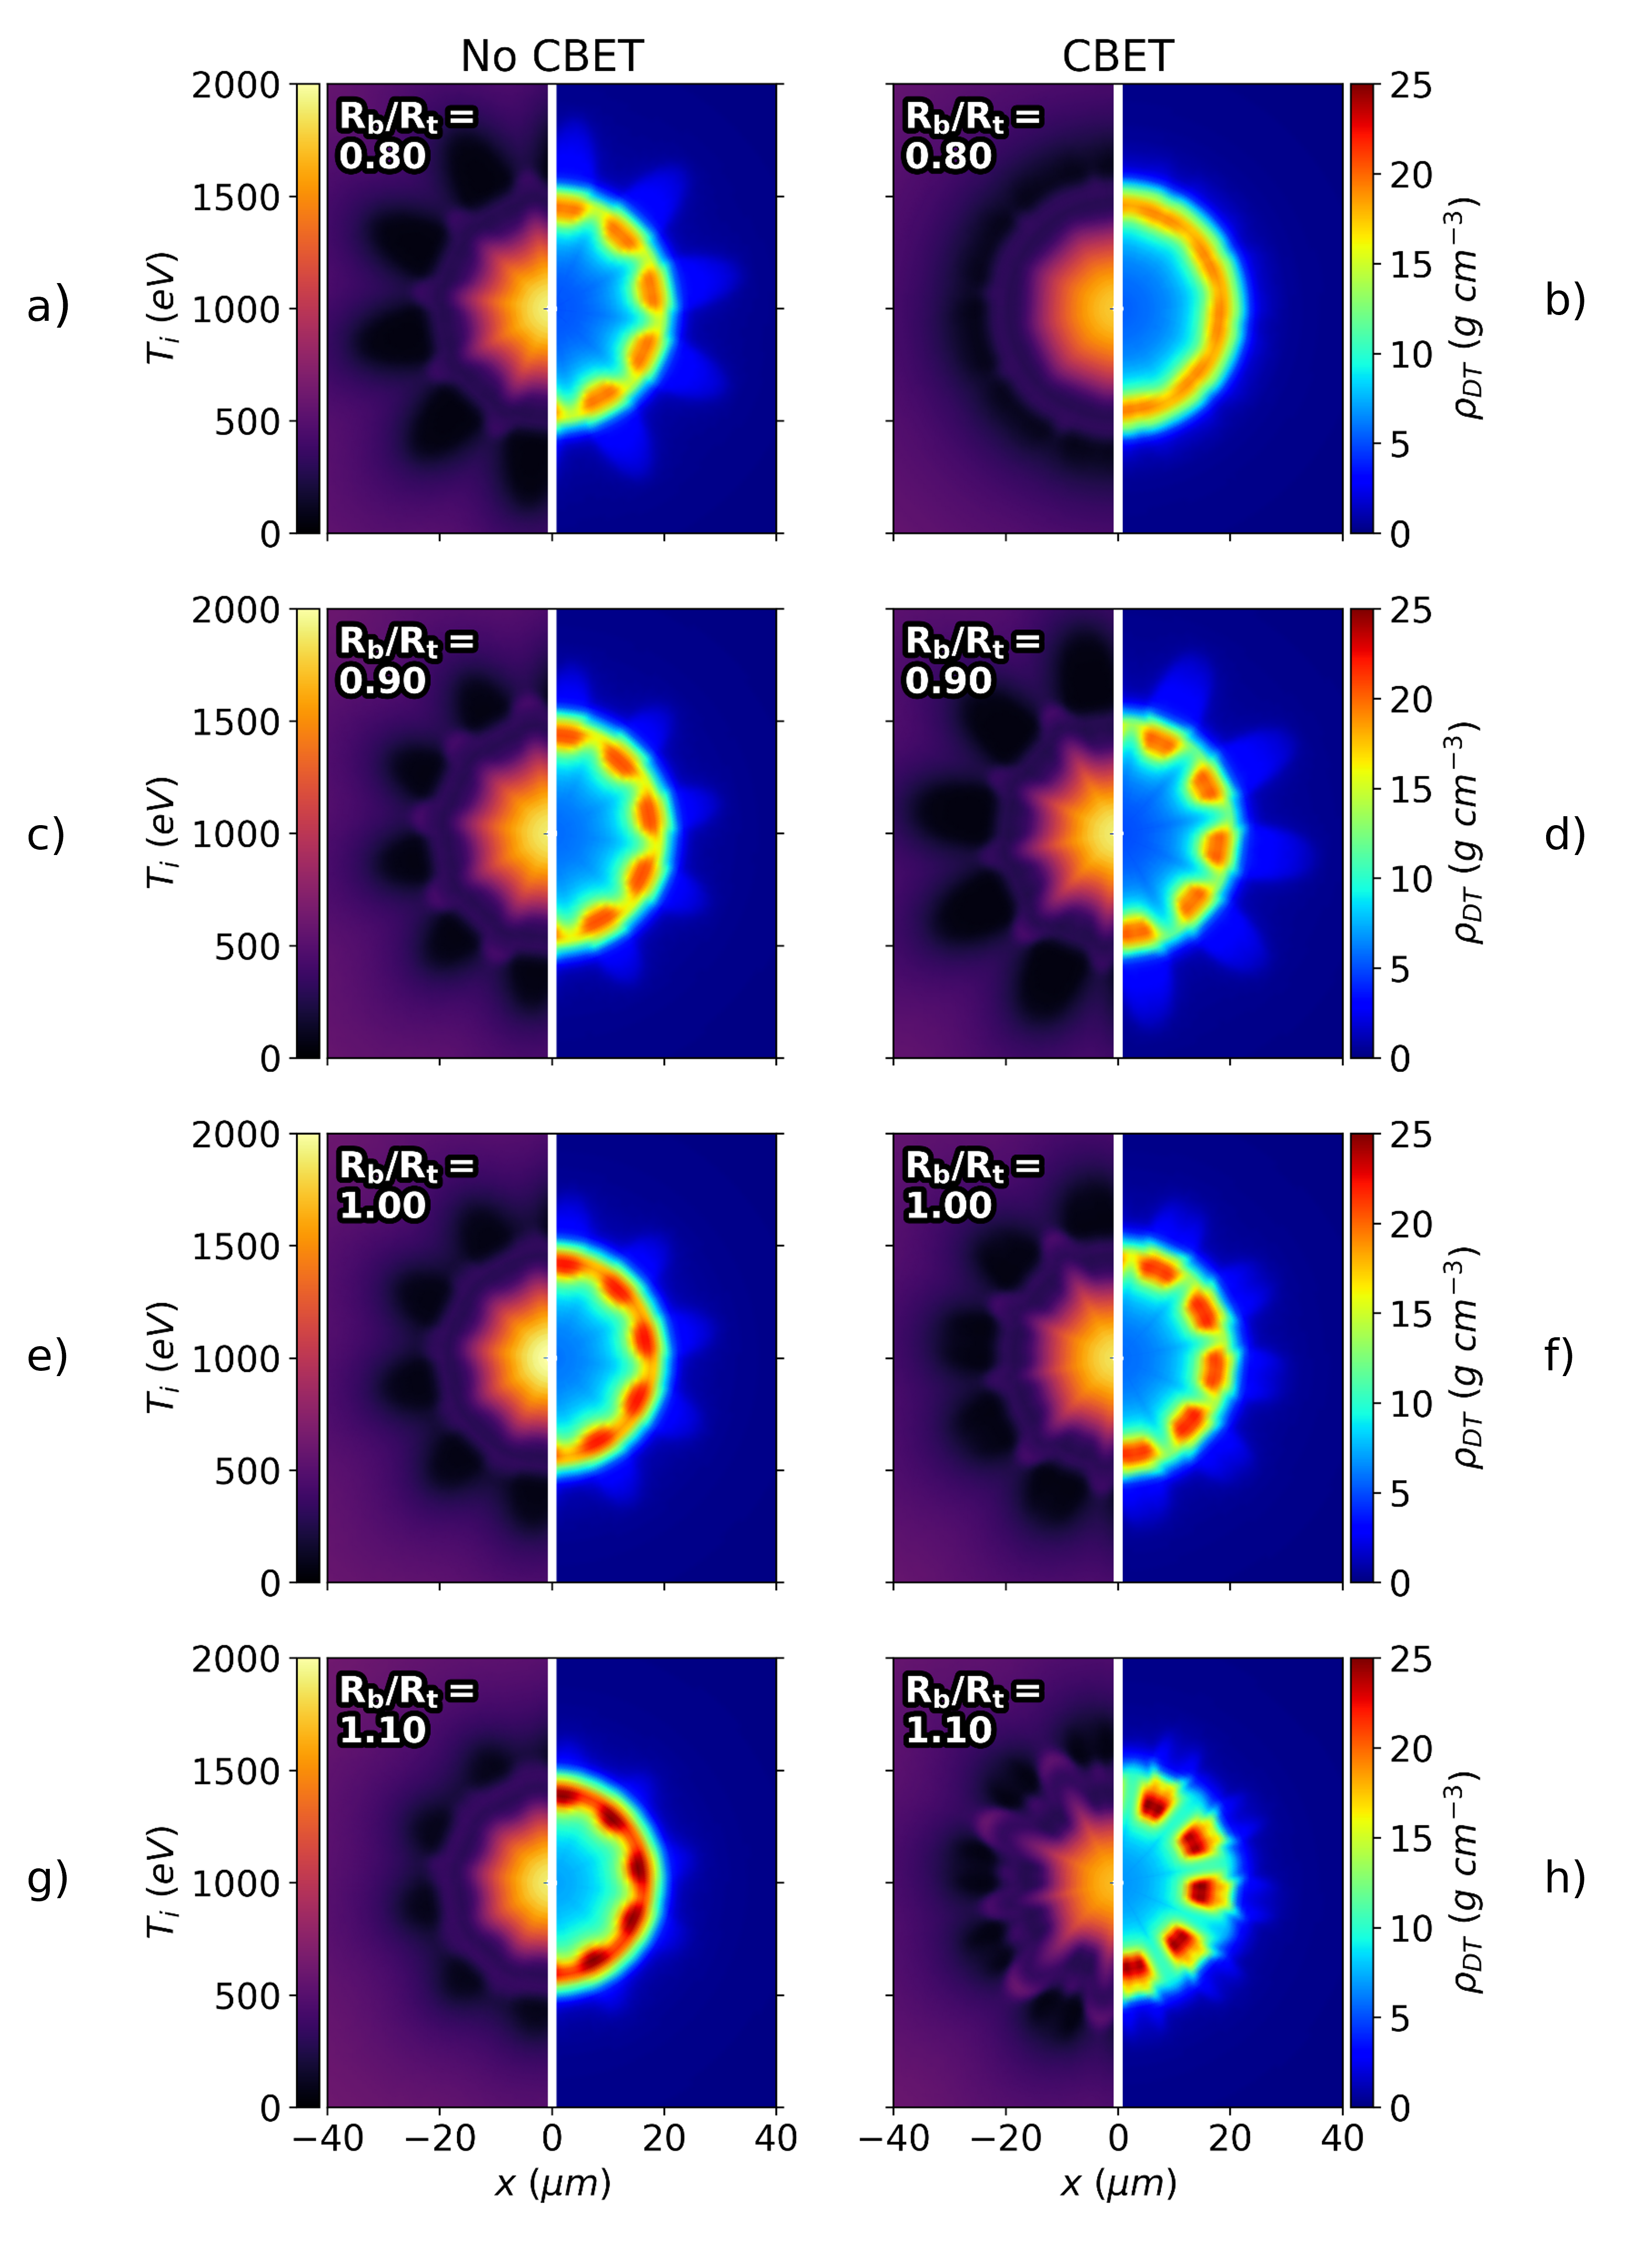
\includegraphics[width=0.9\linewidth]{Results1/Images/Stagnation_plots.png}
    \centering
    \caption{Densities of the DT fuel and ion temperatures for various $R_b/R_t$ simulations both with and without \ac{CBET}.
    Each row correspond to a different $R_b/R_t$ value; the left column contains simulations without \ac{CBET}; and the right column contains simulations with \ac{CBET}.
    It is visible from the density plots that increasing $R_b/R_t$ improves stagnation symmetry for the no-\ac{CBET} simulations, but degrades it for the \ac{CBET} simulations.}%
    \label{fig:Res1_stagnation_plots}
\end{figure}

Fig.~\ref{fig:Res1_stagnation_plots} plots the stagnation fuel density and ion temperature for both the \ac{CBET} and no-\ac{CBET} simulations at 4 different $R_b/R_t$.
The beam-mode $\ell=10$ is clearly identifiable in all plots.
Recall that all simulations are tuned to have the same amount of absorbed laser energy, via the tuning process described in Sec.~\ref{sec:Res1_1D_tuning}.
The no-\ac{CBET} results clearly show a trend of increasing stagnation symmetry with increasing $R_b/R_t$, as expected from the plots in Fig.~\ref{fig:Res1_PR_noCBET_modes}, which showed increasing symmetry of absorption with increasing beam radius.
The pressure of the stagnation state is approximately isobaric, and therefore the temperature profiles are inversely proportional to the density.

Peak densities increase and the radius of stagnation decreases marginally as $R_b/R_t$ decrease.
This improved compression is partially due to increased symmetry providing better compression, but also more optimal shock timing for the larger $R_b/R_t$ implosions also contributes.
As is seen in the streak plots in Fig.~\ref{fig:Res1_streaks}, the tuning process led to the first shock hitting the axis slightly earlier at narrower $R_b/R_t$, than for the larger $R_b/R_t$ implosions.
Although the streak plots are for 1-D with-\ac{CBET} simulations, the same trend is observed for the 2-D with- and without-\ac{CBET} simulations.
The more optimal shock timing for larger $R_b/R_t$ also has the signature of higher on-axis densities.
The contribution of small differences in shock timing is not quantified in the following analysis, but it is assumed that it will have a second order effect on the stagnation symmetry, compared to asymmetry in deposition.

Increasing $R_b/R_t$ when including \ac{CBET} broadly shows the opposite behaviour to the no-\ac{CBET} simulations, exhibiting highly non-uniform density profiles at large $R_b/R_t$.
This trend was also observed in the deposition plots in Fig.~\ref{fig:Res1_PR_CBET_modes}, with the wider beam simulations leading to a more saturated plot on the colour scale.
Higher order modes than $\ell=10$ also become increasingly evident in the wider beam \ac{CBET} simulations.
Note that the $R_b/R_t=0.8$ simulation with \ac{CBET} is more symmetric than the no-\ac{CBET} simulation at the same beam radius.
This is believed to be due to the developing mode-flip in Fig.~\ref{fig:Res1_PR_CBET_modes}.a from $t\sim 0.5\rightarrow 1.3\ \text{ns}$, strongly reducing the absorption asymmetry and subsequent imprinting onto the density early while the capsule is in-flight.

\begin{figure}[t!]
    \includegraphics[width=1.0\linewidth]{Results1/Images/RbRt_sig_rhomax.png}
    \centering
    \caption{Trends of a) stagnation asymmetry and b) maximum (azimuthally averaged) fuel density for \ac{CBET} and no-\ac{CBET} simulations.
    The no-\ac{CBET} improvement in symmetry with $R_b/R_t$ is observed which also corresponds to improved compression.
    The symmetry trend including \ac{CBET} is more complex, but broadly the stagnation state symmetry is worse with increasing $R_b/R_t$.}%
    \label{fig:Res1_asymm_trend}
\end{figure}

The standard deviations of the radially integrated stagnation state fuel density,
\begin{equation}
    \sigma [\rho_{\text{DT}}R] = \sqrt{ \langle \rho_{\text{DT}}R^2 \rangle - \langle \rho_{\text{DT}}R \rangle^2 },
\end{equation}
for the \ac{CBET} and no-\ac{CBET} simulations are plotted as a function of $R_b/R_t$ in Fig.~\ref{fig:Res1_asymm_trend}.a.
The no-\ac{CBET} trend from this metric clearly follow the behaviour seen in Fig.~\ref{fig:Res1_stagnation_plots}, were increasing beam width results in better symmetry of the hydrodynamic profiles at stagnation.
Note that the $R_b/R_t=0.75$ simulation value is more symmetric than the $0.8$ result, suggesting that more complex behaviour may occur at smaller beam radii.
This suggests that more complex symmetry behaviour may occur without \ac{CBET} for $R_b/R_t<0.8$, but this is outside of the range of typical \textsc{Omega} implosions and therefore not studied in detail.
The with-\ac{CBET} curve shows a broad trend of increasing asymmetry with wider beams, as observed from the stagnation profiles in Fig.~\ref{fig:Res1_stagnation_plots}, however the behaviour is clearly more complex than the no-\ac{CBET} simulations.
A local maxima of asymmetry is observed at $R_b/R_t=0.9$ and minima at $R_b/R_t=1.0$.
As shall be described in the subsequent section, Sec.~\ref{sec:Res1_time_res_growth}, these features are explained by the complex, \ac{CBET} induced modal-flips of the deposition which were described in Sec.~\ref{sec:Res1_CBET_asymmetries}.

The azimuthally averaged maximum density,
\begin{equation}
    \rho_{\text{DT,max}} = \text{max}\left( \int_{-\pi}^{\pi} \rho_{\text{DT}}(r,\phi)\ \text{d}\phi \right),
\end{equation}
is plotted in Fig.~\ref{fig:Res1_asymm_trend}.b for both sets of simulations.
The behaviour in this plot is inversely proportional to the standard deviation, which suggests that the asymmetry of the density has a detrimental effect on the compression of the target.
The (unintended) improved shock timing at larger beam radii does appear to somewhat compensate for the reduction in uniformity, \textit{i.e.} the compression metric at $R_b/R_t=1.05$ is about the same as $R_b/R_t=0.8$, despite far worse symmetry.
It is therefore, difficult to quantify the contribution to the degradation of compression due to each of these effects, from this set of simulations.

%################################################################################
%################################################################################
\subsection{Time Resolved Asymmetry Growth}%
\label{sec:Res1_time_res_growth}

\begin{figure}[t!]
    \includegraphics[width=0.75\linewidth]{Results1/Images/RbRts_mode10_growth.png}
    \centering
    \caption{Time resolved $\ell=10$ Fourier power spectrum amplitude for a) $\rho_{\text{DT}}R$ and b) $P_{\text{dep}}R$ for \ac{CBET} simulations with 3 $R_b/R_t$ values.
    The developing but unrealised modal flip for $R_b/R_t=0.8$ from $t \sim 0.5\rightarrow 1.2\ \text{ns}$ reduces the $P_{\text{dep}}R_{\ell=10}$ leading to slow $\rho_{\text{DT}}R_{\ell=10}$ growth and ultimately a relatively symmetric stagnation state.
    %Note that this developing but unrealised modal flip is clearly visible from reduced $P_{\text{dep}}R$ asymmetry values in Fig.~\ref{fig:Res1_PR_CBET_modes}.a.
    Despite large values of $\rho_{\text{DT}}R_{\ell=10}$ initially, the developing modal flip of the $R_b/R_t=1.0$ simulation from $t \sim 1.8\rightarrow 2.1\ \text{ns}$ slows the density asymmetry growth.}%
    \label{fig:Res1_mode10_growths}
\end{figure}

asym growth time res


%###############################################################################################################################
%###############################################################################################################################
%###############################################################################################################################
\section{Conclusions}%
\label{sec:Res1_Conclusions}

conlusions

%################################################################################
%################################################################################
\subsection{Summary of work}%
\label{sec:Res1_Summary}

summary

%################################################################################
%################################################################################
\subsection{Future Work}%
\label{sec:Res1_future}

future